\noindent
{\Large \textbf{\section{Результаты работы}}} \par

\noindent{\Large \textbf{\subsection{Работа программы на случайных начальных условиях}}} \par

На рис.\ref{fig:random} показаны начальное состояние и первые три итерации работы программы на случайном поле $10\times 10$. Из начального «шума» за несколько шагов формируются регулярные фрагменты, похожие на диагональные полосы.
\begin{figure}[H]
 \centering
 \begin{minipage}{0.48\textwidth}
  \centering
  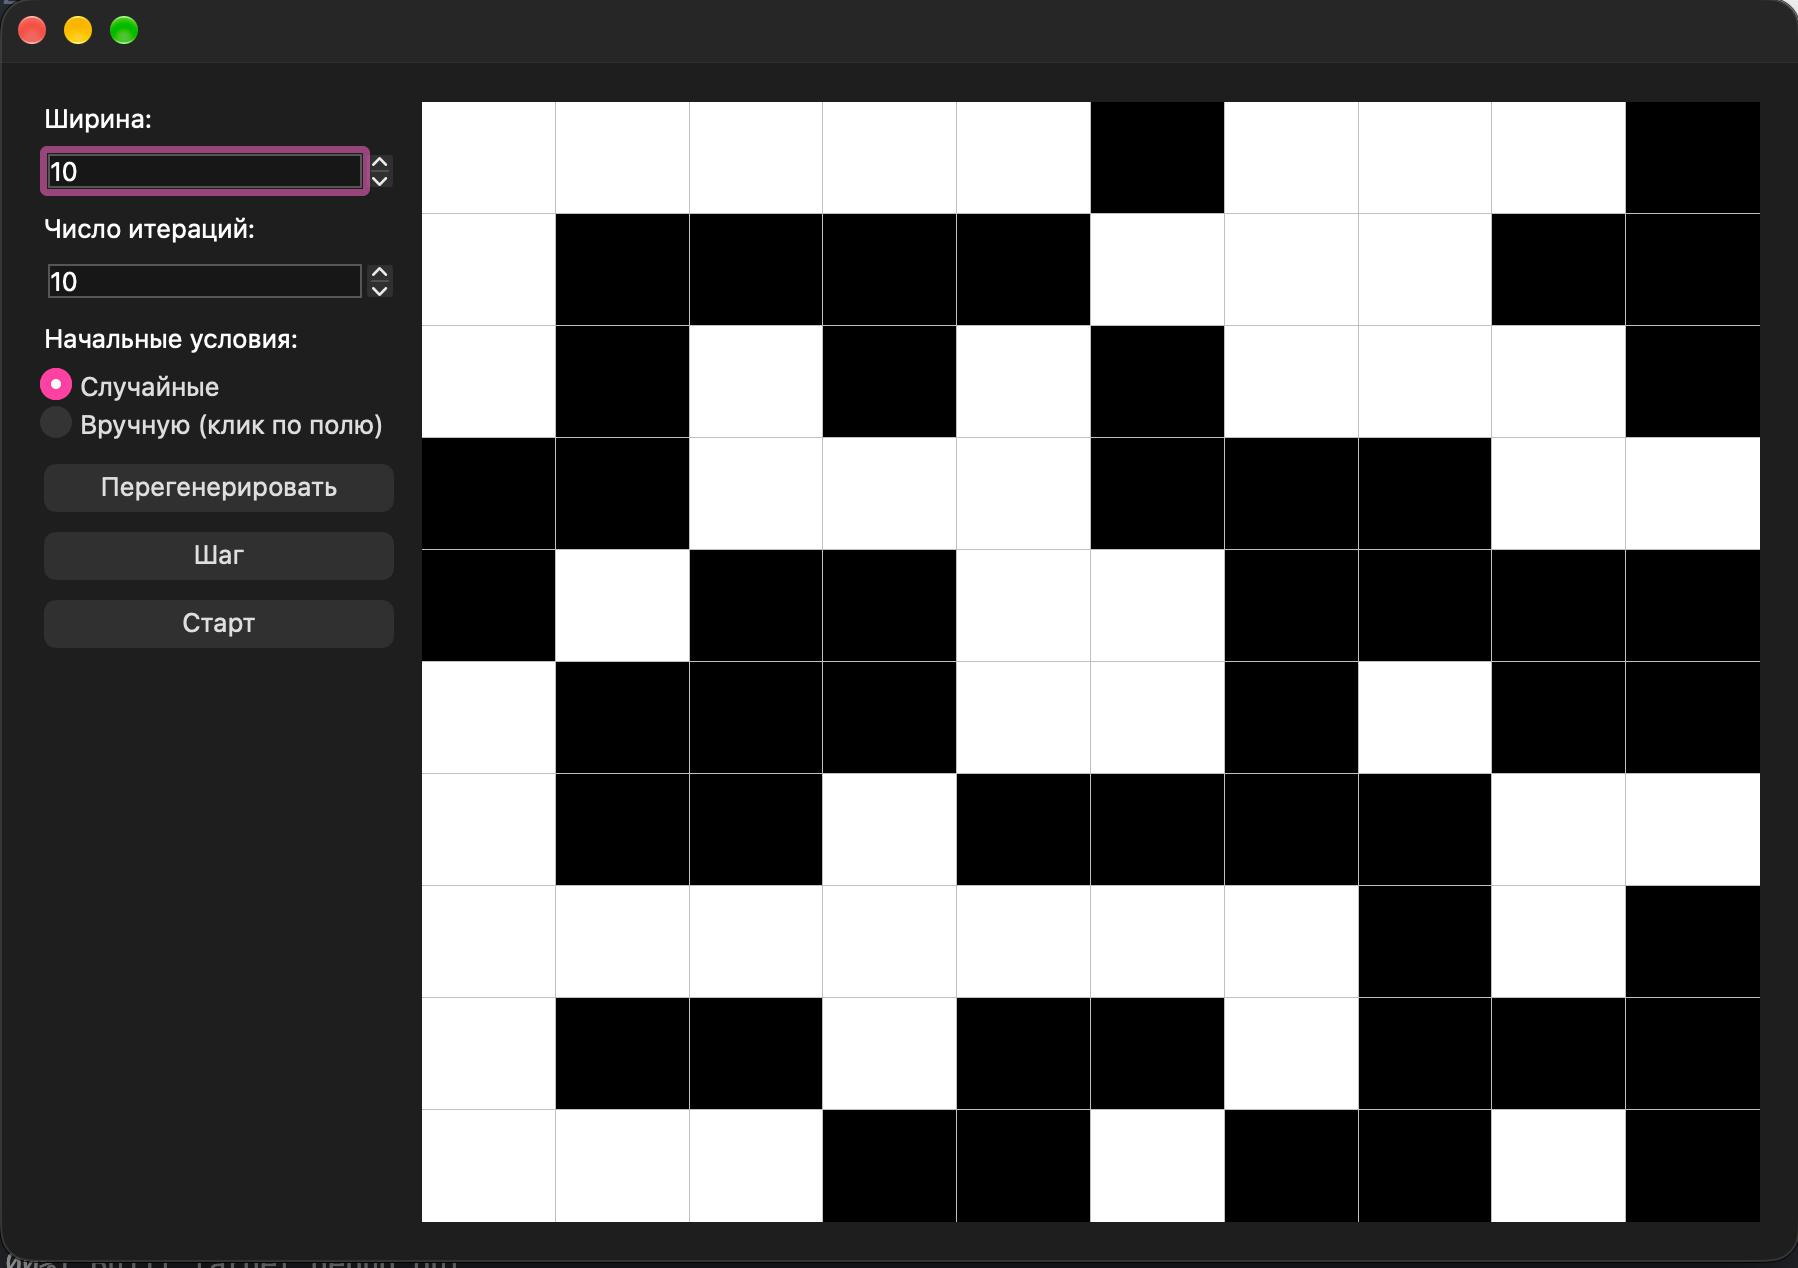
\includegraphics[width=\textwidth]{pic/random_t0.jpg}\\
  а) $t=0$ (начальное состояние)
 \end{minipage}
 \hfill
 \begin{minipage}{0.48\textwidth}
  \centering
  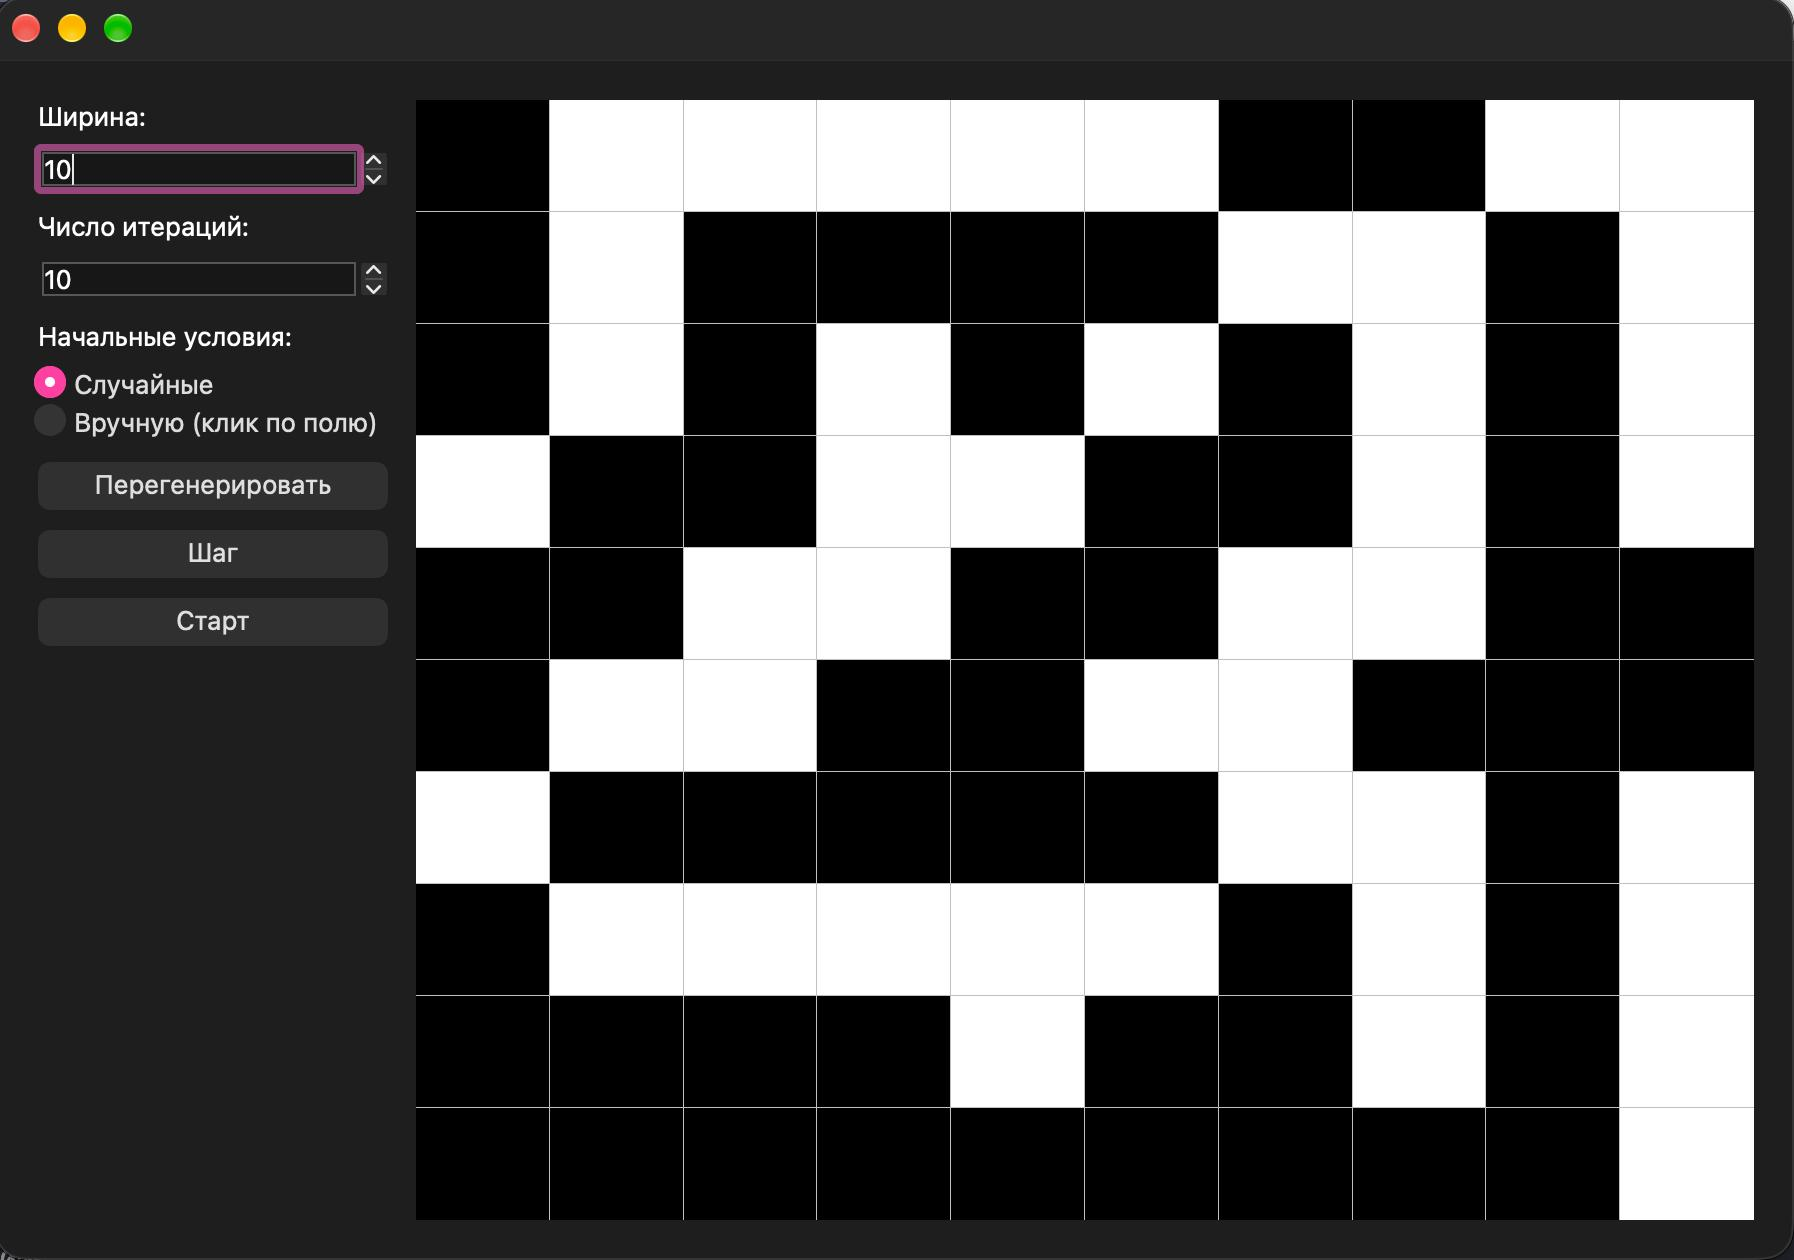
\includegraphics[width=\textwidth]{pic/random_t1.jpg}\\
  б) $t=1$
 \end{minipage}

 \vspace{0.5cm}

 \begin{minipage}{0.48\textwidth}
  \centering
  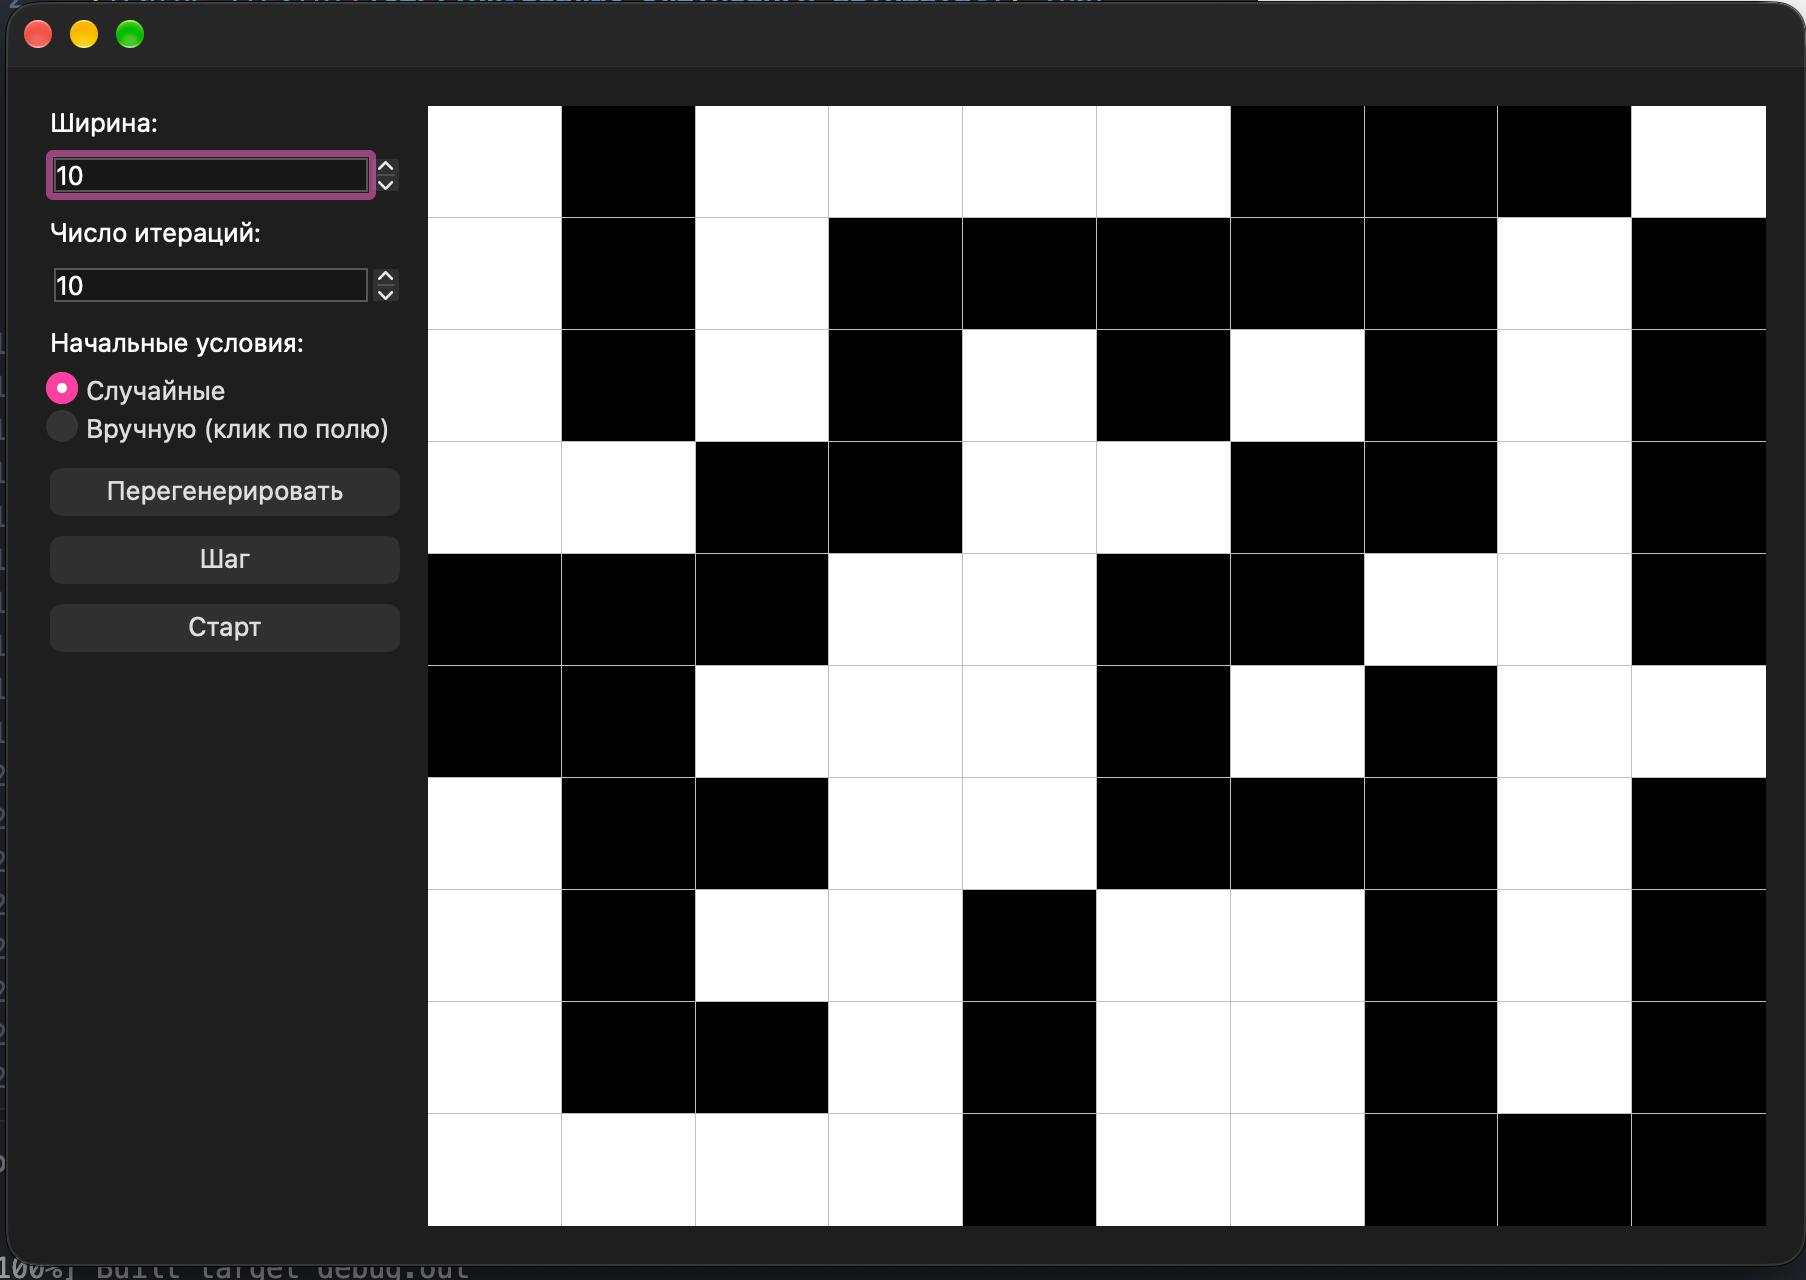
\includegraphics[width=\textwidth]{pic/random_t2.jpg}\\
  в) $t=2$
 \end{minipage}
 \hfill
 \begin{minipage}{0.48\textwidth}
  \centering
  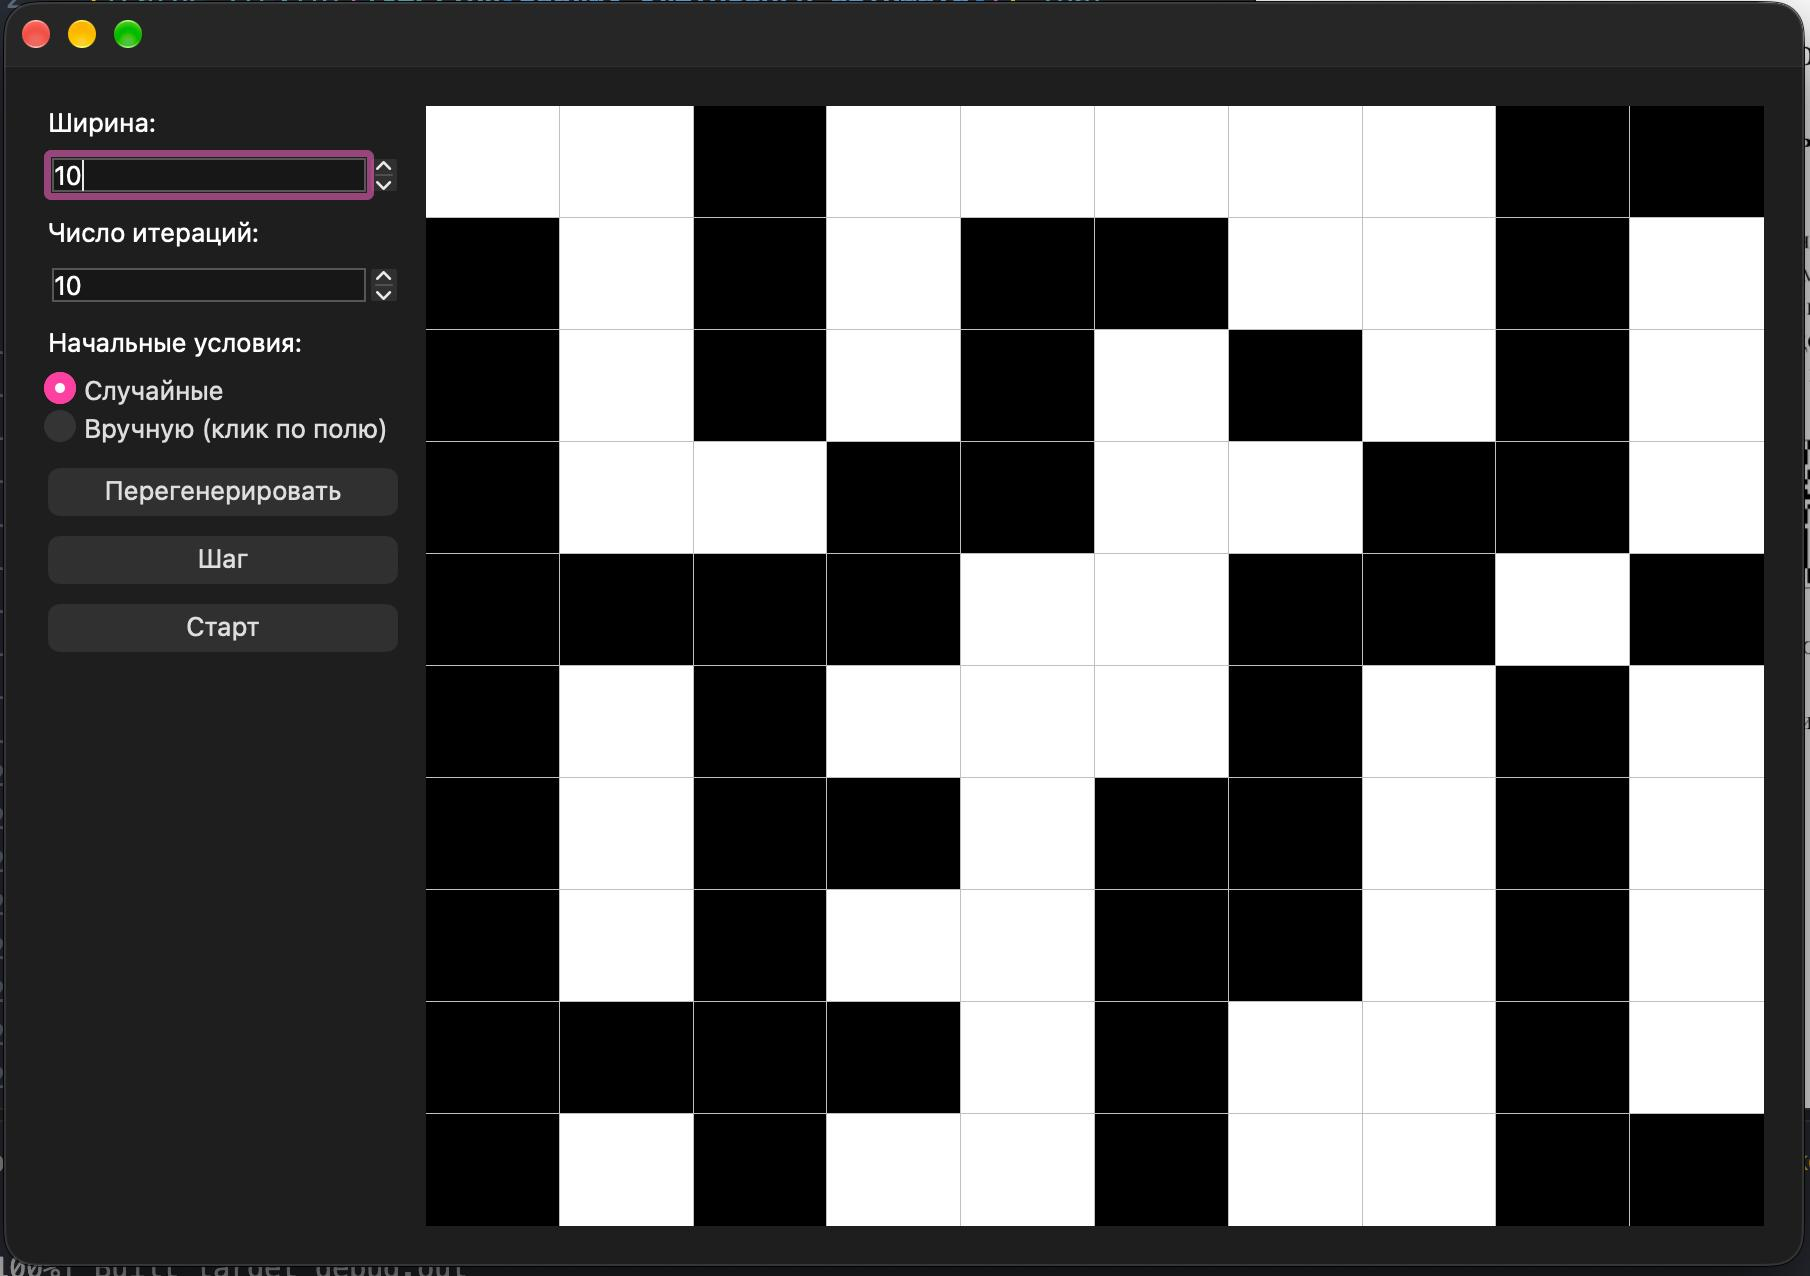
\includegraphics[width=\textwidth]{pic/random_t3.jpg}\\
  г) $t=3$
 \end{minipage}
 \caption{Первые три итерации на случайном поле $10\times 10$}
 \label{fig:random}
\end{figure}

\noindent{\Large \textbf{\subsection{Работа программы на ручных начальных условиях}}} \par

На рис.\ref{fig:manual} показаны начальное состояние, заданное вручную кликами по полю $10\times 10$, и первые пять итераций.

\begin{figure}[H]
 \centering
 \begin{minipage}{0.48\textwidth}
  \centering
  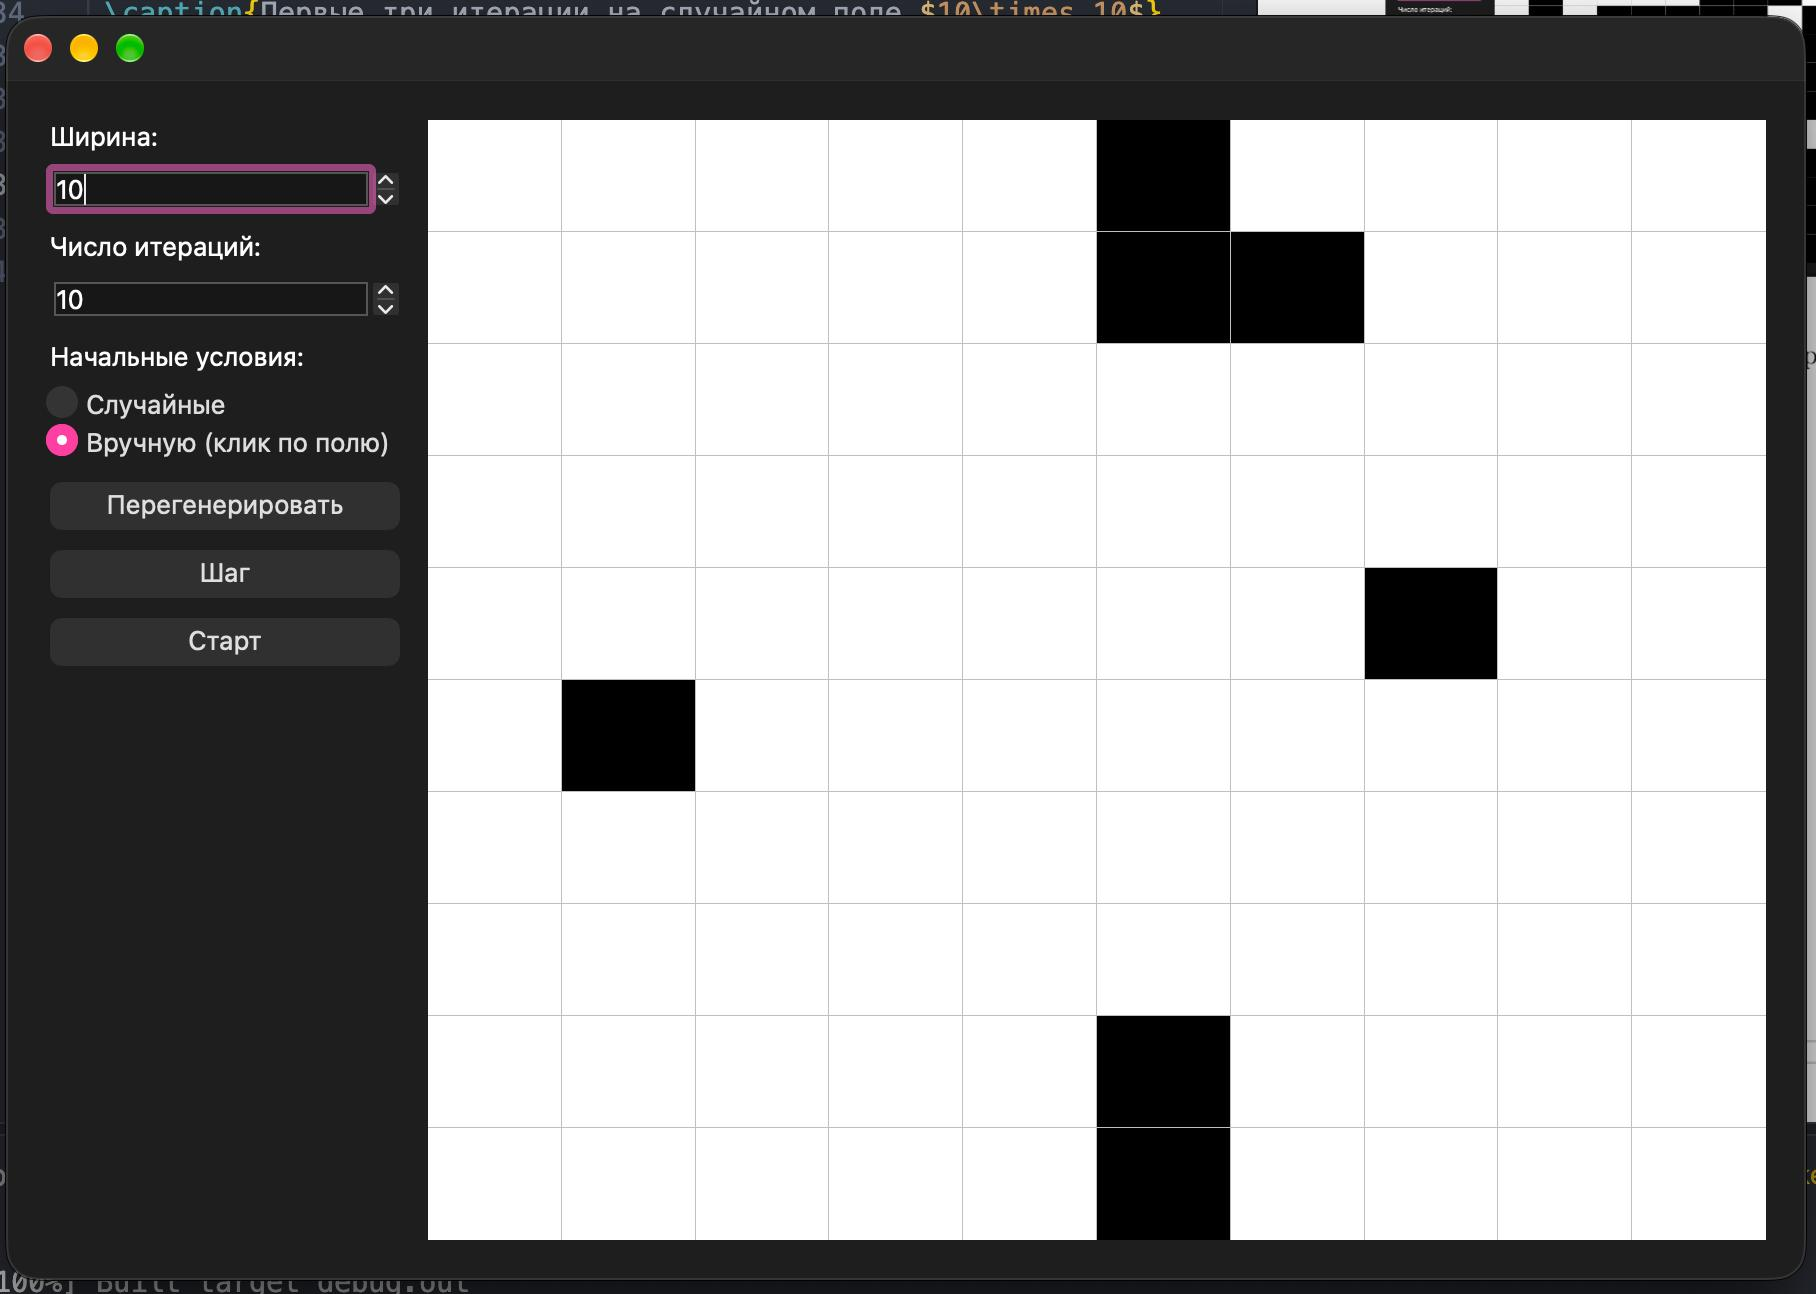
\includegraphics[width=\textwidth]{pic/manual_t0.jpg}\\
  а) $t=0$ (начальное состояние)
 \end{minipage}
 \hfill
 \begin{minipage}{0.48\textwidth}
  \centering
  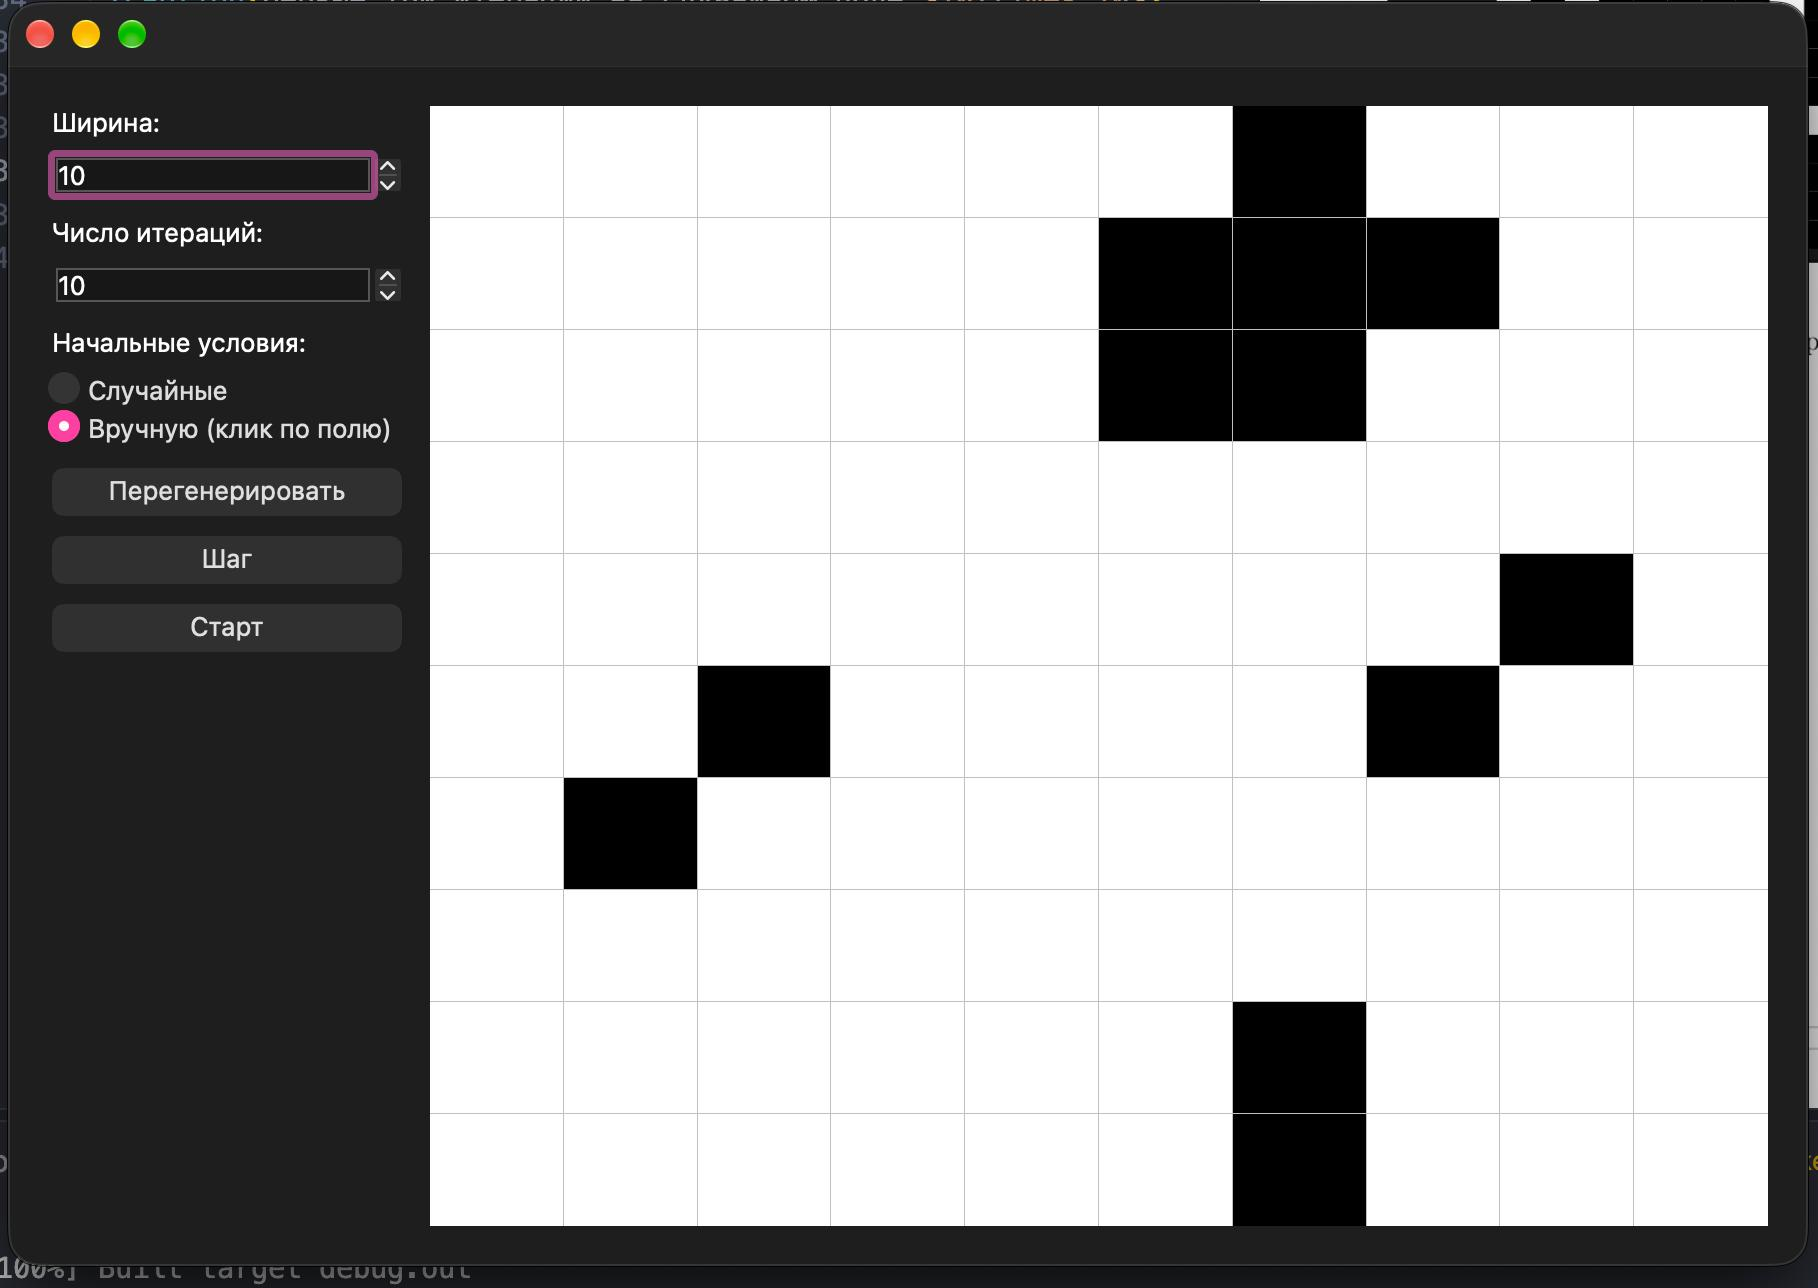
\includegraphics[width=\textwidth]{pic/manual_t1.jpg}\\
  б) $t=1$
 \end{minipage}

 \vspace{0.3cm}

 \begin{minipage}{0.48\textwidth}
  \centering
  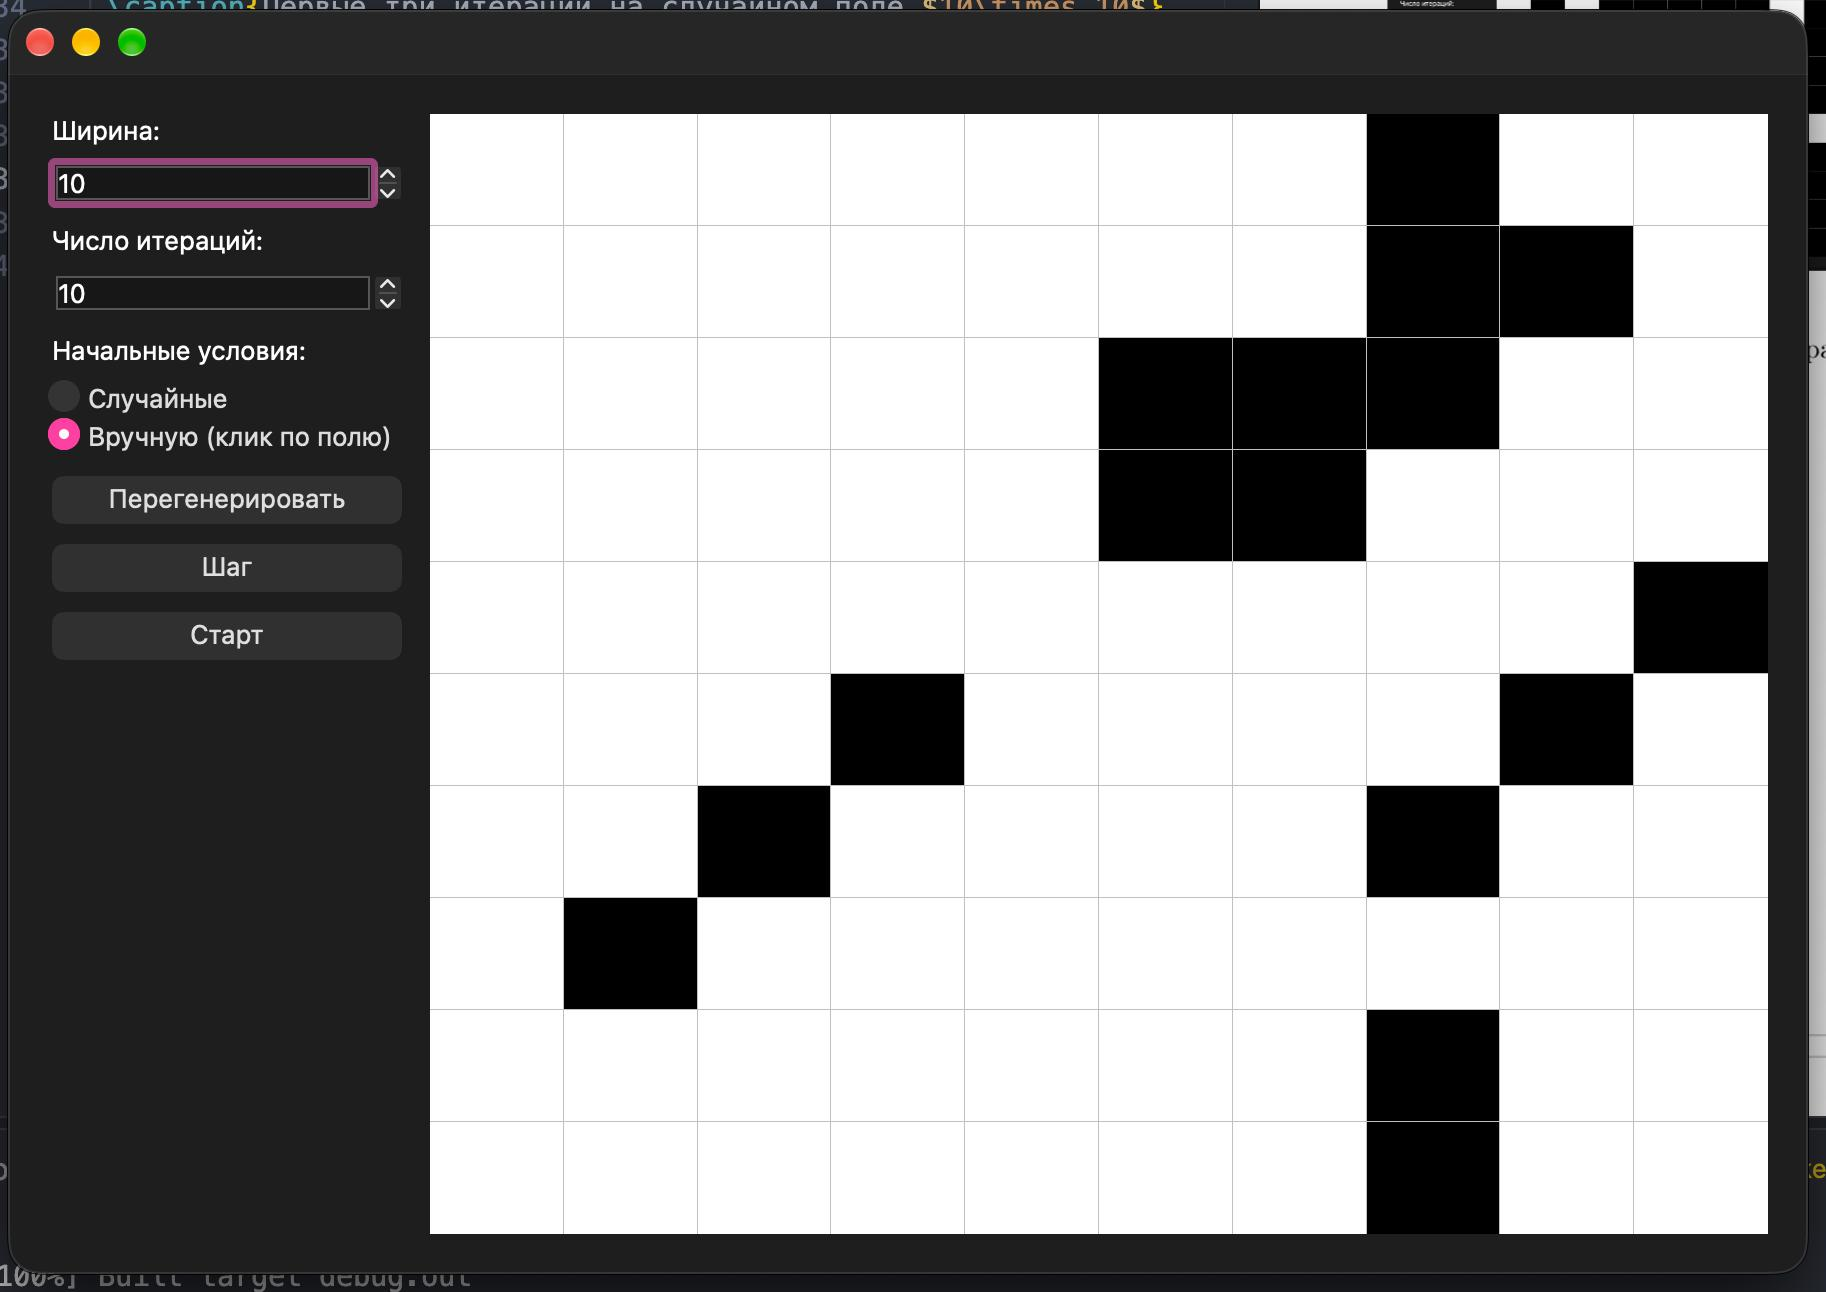
\includegraphics[width=\textwidth]{pic/manual_t2.jpg}\\
  в) $t=2$
 \end{minipage}
 \hfill
 \begin{minipage}{0.48\textwidth}
  \centering
  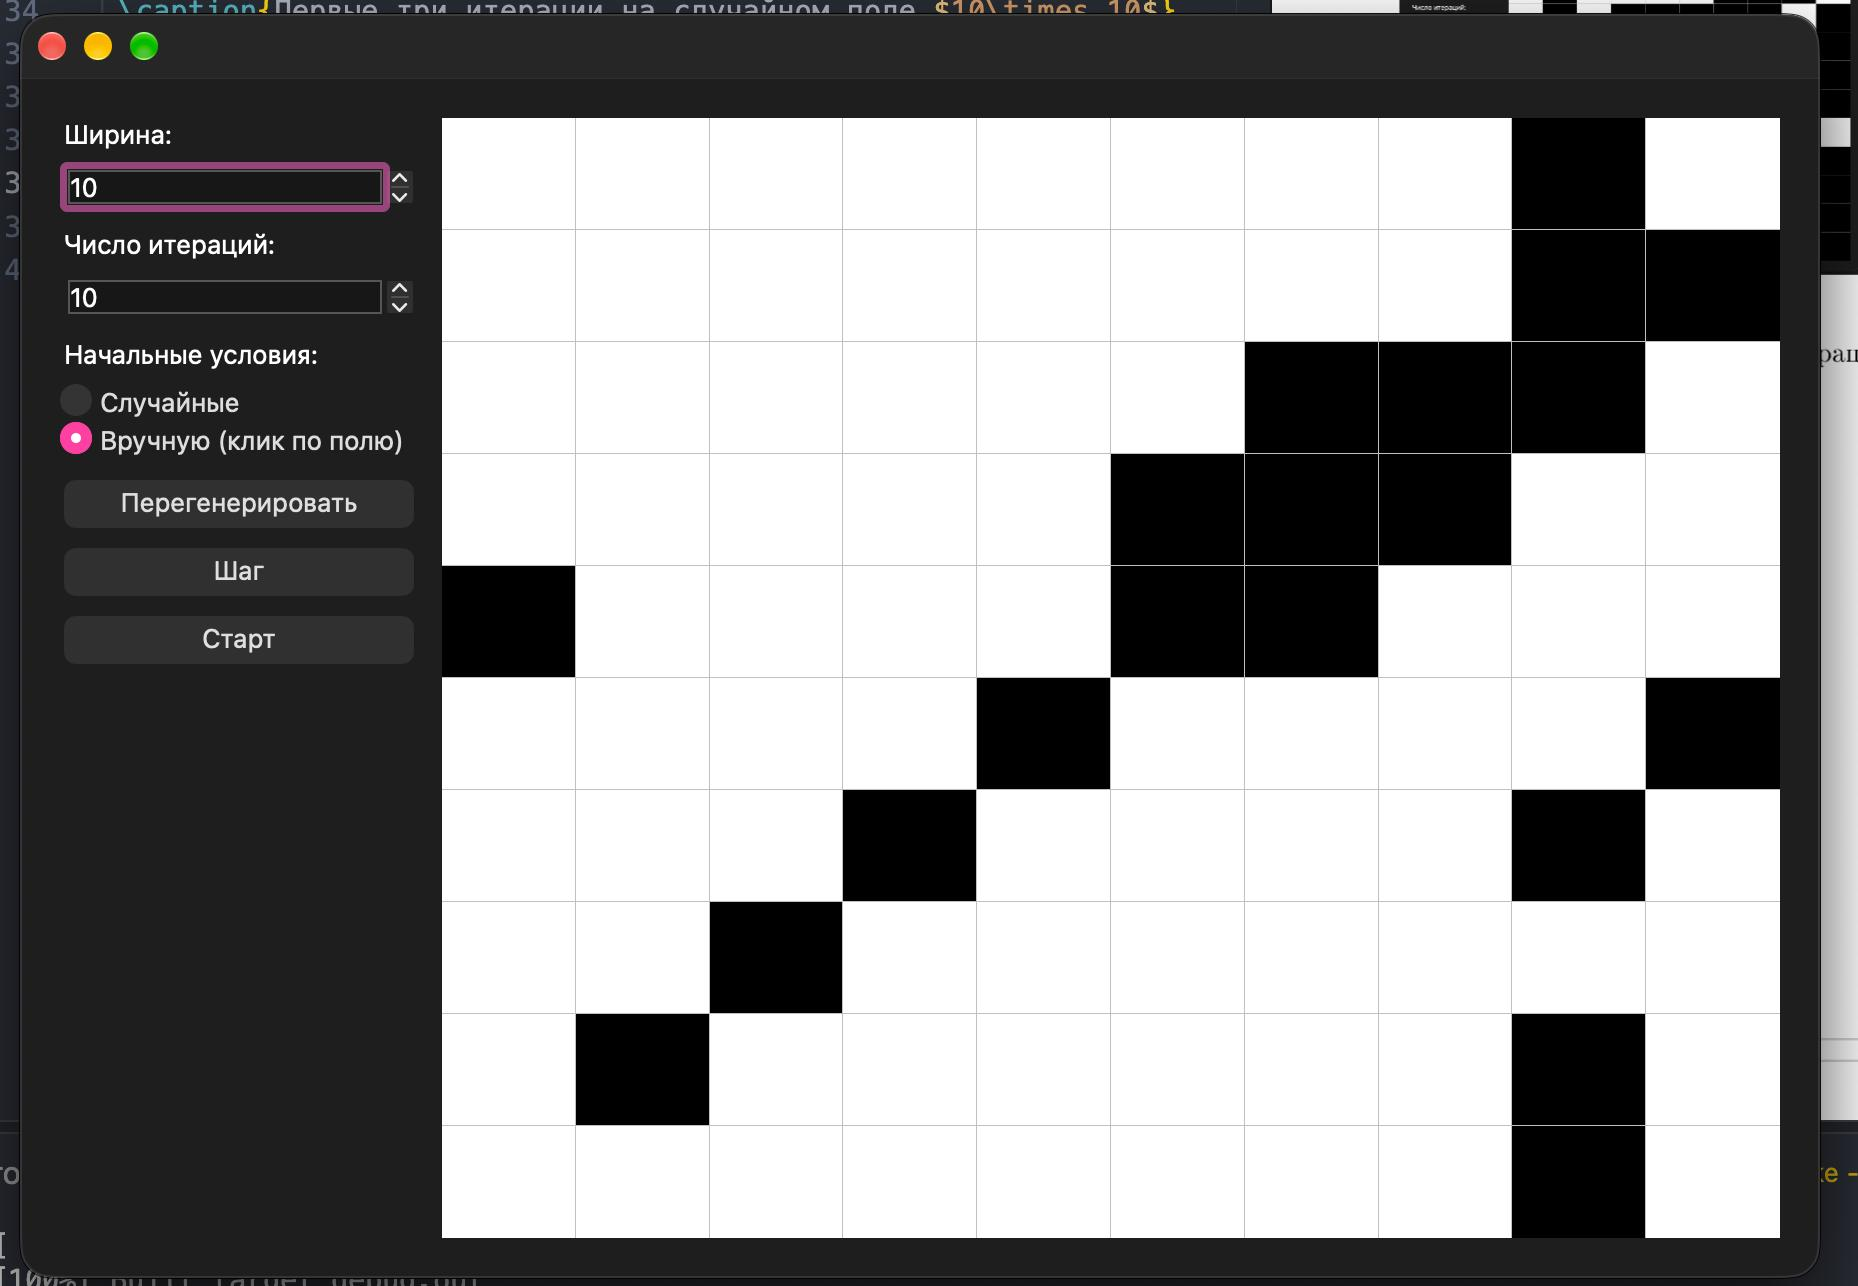
\includegraphics[width=\textwidth]{pic/manual_t3.jpg}\\
  г) $t=3$
 \end{minipage}

 \vspace{0.3cm}

 \begin{minipage}{0.48\textwidth}
  \centering
  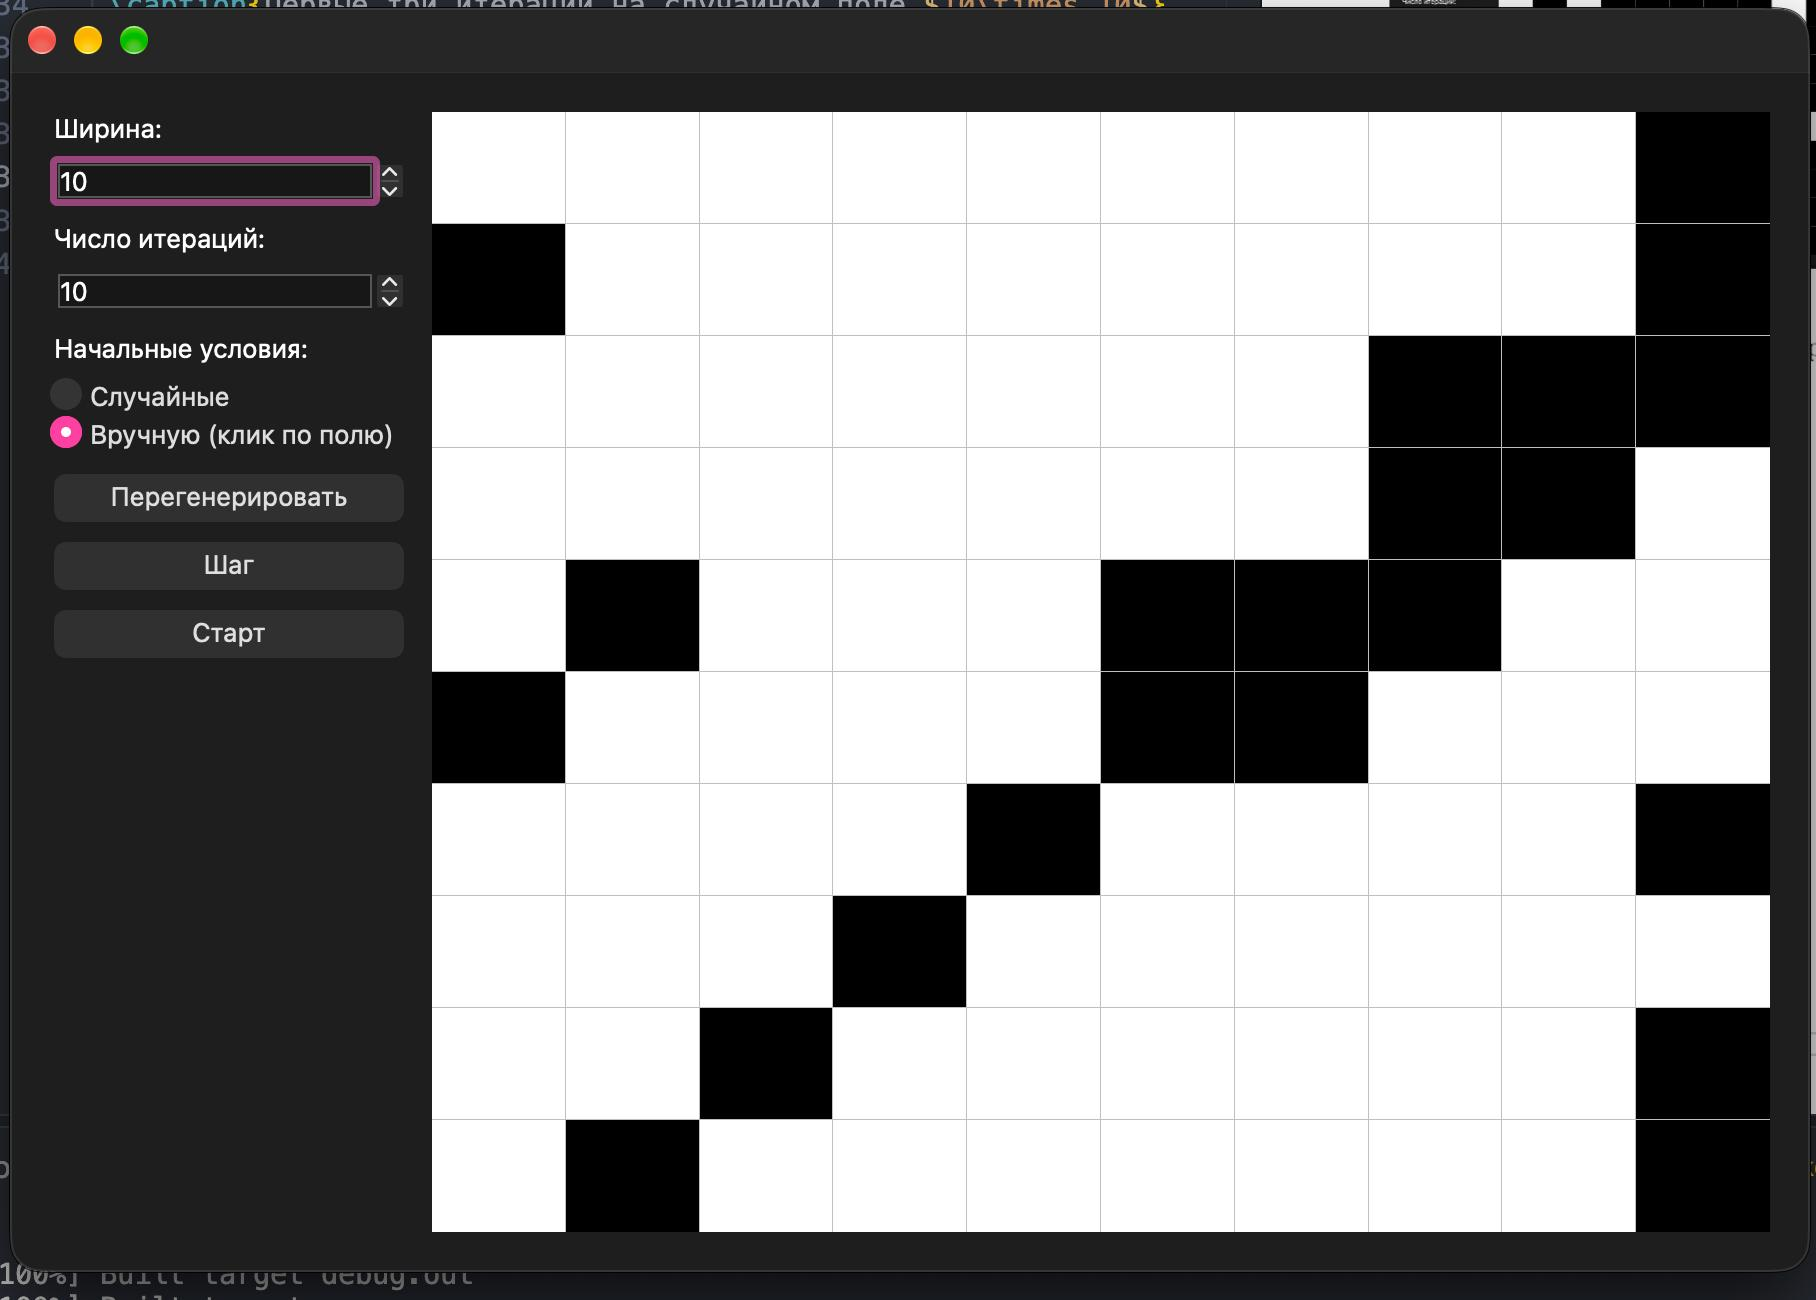
\includegraphics[width=\textwidth]{pic/manual_t4.jpg}\\
  д) $t=4$
 \end{minipage}
 \hfill
 \begin{minipage}{0.48\textwidth}
  \centering
  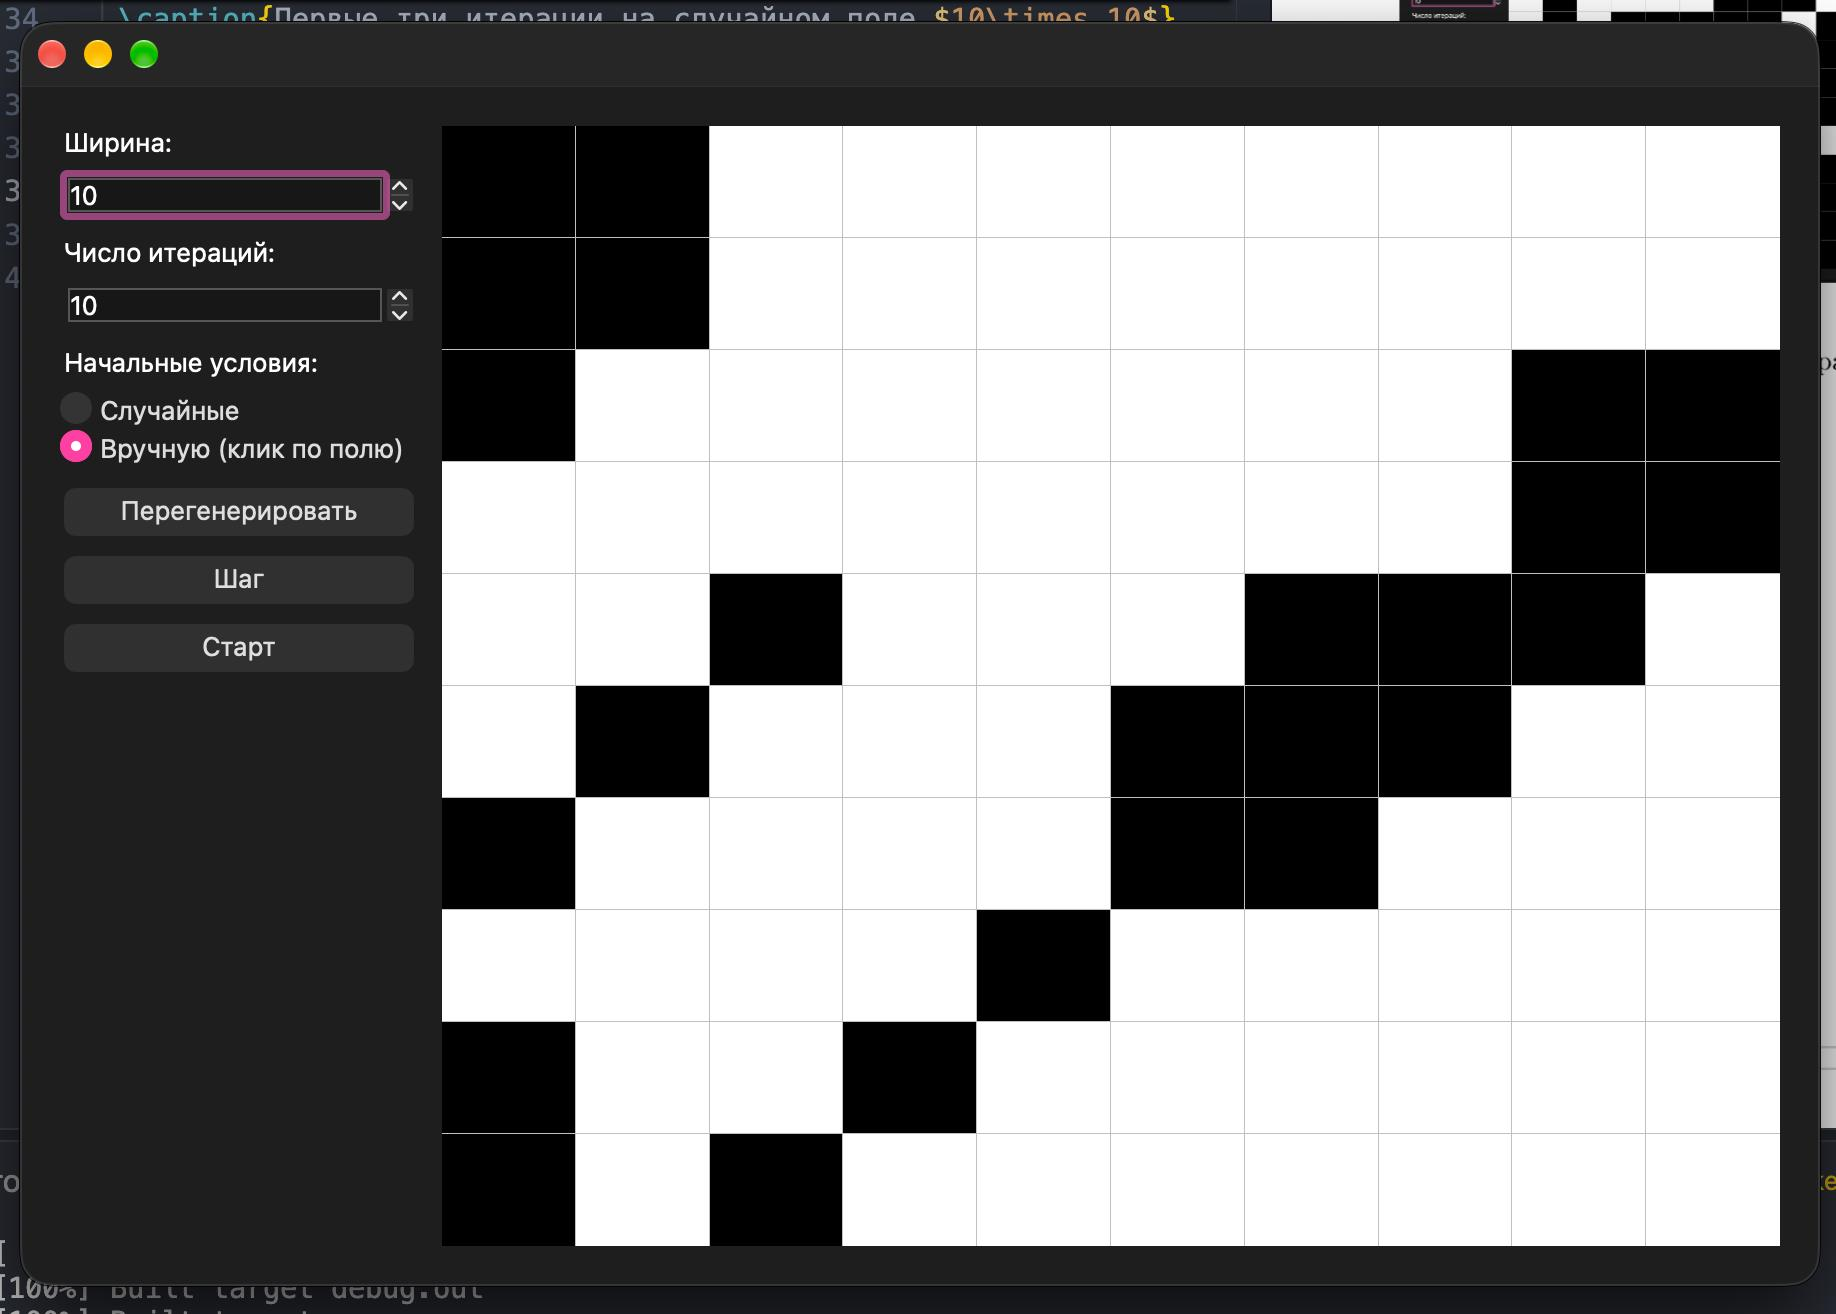
\includegraphics[width=\textwidth]{pic/manual_t5.jpg}\\
  е) $t=5$
 \end{minipage}
 \caption{Первые пять итераций при ручных начальных условиях, поле $10\times 10$}
 \label{fig:manual}
\end{figure}

\newpage
